\documentclass[t]{beamer}
\mode<presentation>

\usepackage{palatino} % Uncomment to use the Palatino font

\usepackage{graphicx} % Required for including images
\graphicspath{{figures/}} % Location of the graphics files
\usepackage{booktabs} % Top and bottom rules for table
\usepackage[font=small,labelfont=bf]{caption} % Required for specifying captions to tables and figures
\usepackage{wrapfig} % Allows wrapping text around tables and figures
\usepackage{lipsum,adjustbox}
\usepackage[absolute,overlay]{textpos}
\usepackage{url}
\usepackage{lmodern}
\usepackage{amsmath}
\usepackage{amsfonts}
\usepackage{color}
\usepackage{array}
\usepackage{multirow}
\usepackage{multicol}
\usepackage{tikz}
\usepackage{tikz-dependency}
\usetikzlibrary{arrows.meta,graphs,graphs.standard,graphdrawing,quotes,shapes}
\usegdlibrary{layered}
\captionsetup{labelformat=empty}
\newcommand{\parser}[1]{TUPA\textsubscript{#1}}

\makeatletter
\pgfdeclareshape{vector}{
	  \inheritsavedanchors[from={rectangle}]
	  \inheritbackgroundpath[from={rectangle}]
	  \inheritanchorborder[from={rectangle}]
	  \foreach \x in {center,north east,north west,north,south,south east,south west,east,west}{
	    \inheritanchor[from={rectangle}]{\x}
	  }

    \backgroundpath{
      \pgftransformshift{\pgfpoint{-16pt}{-4pt}}
		  \draw[rounded corners=2pt] (0,0) rectangle (32pt,8pt);
    }

    \beforebackgroundpath{
      \draw[step=8pt,help lines,-] (8pt,.1pt) grid (24pt,7.9pt);
    }
}
\makeatother


\begin{document}


\title[A Transition-Based DAG Parser for UCCA]{A Transition-Based Directed Acyclic Graph Parser for Universal Conceptual Cognitive Annotation}
\author{Daniel Hershcovich, Omri Abend and Ari Rappoport}
\institute[]{
\includegraphics[width=.08\pagewidth]{huji_logo.jpg}

\includegraphics[width=.3\pagewidth]{huji_banner.png}}
\date{ACL 2017}

\begin{frame}
\titlepage
\end{frame}


%----------------------------------------------------------------------------------------

\section{Universal Conceptual Cognitive Annotation}

\begin{frame}
\frametitle{Universal Conceptual Cognitive Annotation (UCCA)}
\begin{tikzpicture}[level distance=25mm, sibling distance=23mm, ->,
    every circle node/.append style={fill=black},
    every node/.append style={font=\rmfamily}]
  \node (ROOT) [circle] {}
    child {node (After) {After} edge from parent node[left] {$L$}}
    child {node (graduation) [circle] {}
    {
      child {node {graduation} edge from parent node[left] {$P$}}
    } edge from parent node[left] {$H$} }
    child {node {,} edge from parent node[right] {$U$}}
    child {node (moved) [circle] {}
    {
      child {node (John) {John} edge from parent node[left] {$A$}}
      child {node {moved} edge from parent node[left] {$P$}}
      child {node [circle] {}
      {
        child {node {to} edge from parent node[left] {$R$}}
        child {node {Paris} edge from parent node[right] {$C$}}
      } edge from parent node[right] {$A$} }
    } edge from parent node[right] {$H$} }
    ;
  \draw[dashed,->] (graduation) to node [auto] {$A$} (John);
  \node at (5.6,-.3) {\Large ----- primary edge};
  \node at (5.6,-1.3) {\Large - - - remote edge};
\end{tikzpicture}
\begin{wraptable}{l}{1cm}
  \vspace{-3cm}
  \begin{adjustbox}{margin=1mm,frame}
  \scalebox{.9}{
  \begin{tabular}{c>{\small\it}l|c>{\small\it}l|c>{\small\it}l}
	  $P$ & process &
	  $S$ & state &
	  $A$ & participant \\
	  $L$ & linker &
	  $H$ & linked scene &
	  $C$ & center \\
	  $E$ & elaborator &
	  $D$ & adverbial &
	  $R$ & relator \\
	  $N$ & connector &
	  $U$ & punctuation &
	  $F$ & function \\
	  $G$ & ground
  \end{tabular}
  }
  \end{adjustbox}
\end{wraptable}
\end{frame}

\begin{frame}
\frametitle{Universal Conceptual Cognitive Annotation (UCCA)}
Semantic representation scheme \cite{abend2013universal}
based on typological and Cognitive Linguistics literature \cite{Dixon:basic,croft2004cognitive}.
\begin{itemize}
 \item Demonstrated applicability to English, French, German \& Czech.
 \item Support for rapid annotation.
 \pause
 \item Stability in translation \cite{sulem2015conceptual}.
 \item Useful for MT evaluation \cite{birch2016hume}.
 \item Applicability so far limited by absence of parser.
\end{itemize}

\vfill
\begin{center}
  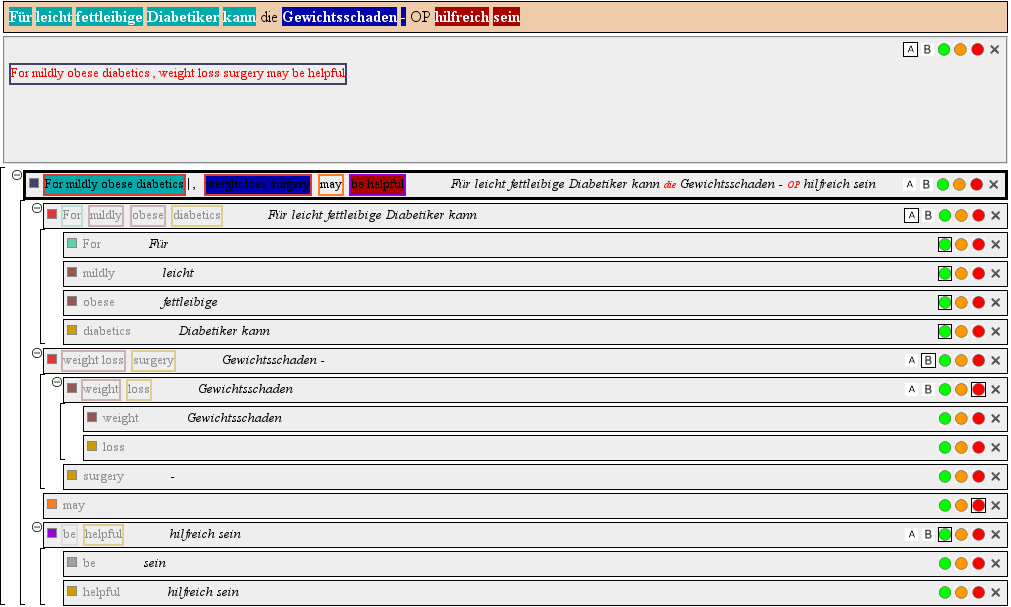
\includegraphics[width=\linewidth]{hume.png}
\end{center}
\end{frame}

\begin{frame}
\frametitle{Universal Conceptual Cognitive Annotation (UCCA)}
\begin{itemize}
 \item \textbf{Remote edges} represent implied relations, allow argument sharing.
 \item The foundational layer covers predicate-argument structure, relations between predicates,
and other constructions such as coordination and multi-word expressions.
 \item Extensible to allow other distinctions.
\end{itemize}
\end{frame}

\begin{frame}
\frametitle{Structural Properties}
\noindent
(1) non-terminal nodes, (2) reentrancy, (3) discontinuity
\centering
\begin{minipage}{.4\linewidth}{\centering
  \begin{tikzpicture}[level distance=12mm, sibling distance=16mm, ->,
      every node/.append style={midway,font=\rmfamily}]
    \node (ROOT) [fill=black, circle] {}
      child {node [fill=black, circle] {}
      {
        child {node {John} edge from parent node[left] {\scriptsize $C$}}
        child {node {and} edge from parent node[left] {\scriptsize $N$}}
        child {node {Mary} edge from parent node[left] {\scriptsize $C$}}
      } edge from parent node[left] {\scriptsize $A$} }
      child {node {went} edge from parent node[left] {\scriptsize $P$}}
      child {node {home} edge from parent node[left] {\scriptsize $A$}}
      ;
  \end{tikzpicture}
  }
\end{minipage}
\hfill
\begin{minipage}{.4\linewidth}{\centering
  \begin{tikzpicture}[level distance=12mm, sibling distance=2cm, ->,
      every node/.append style={midway,font=\rmfamily}]
    \node (ROOT) [fill=black, circle] {}
      child {node {John} edge from parent node[left] {\scriptsize $A$}}
      child {node [fill=black, circle] {}
      {
      	child {node {gave} edge from parent node[left] {\scriptsize $C$}}
      	child {node (everything) {everything} edge from parent[white]}
      	child {node {up} edge from parent node[left] {\scriptsize $C$}}
      } edge from parent node[right] {\scriptsize $P$} }
      ;
    \draw[bend right,->] (ROOT) to[out=-20, in=180] node [left] {\scriptsize $A$} (everything);
  \end{tikzpicture}
  }
\end{minipage}

\vspace{-1mm}
  \begin{tikzpicture}[level distance=12mm, sibling distance=2cm, ->,
      every node/.append style={midway,font=\rmfamily}]
    \node (ROOT) [fill=black, circle] {}
      child {node (John) {John} edge from parent node[left] {\scriptsize $A$}}
      child {node {decided} edge from parent node[left] {\scriptsize $P$}}
      child {node (totakeaquickshower) [fill=black, circle] {}
      {
        child {node {to} edge from parent node[left] {\scriptsize $F$}}
        child {node (takeashower) [fill=black, circle] {}
        {
          child {node {take} edge from parent node[left] {\scriptsize $C$}}
          child {node {a} edge from parent node[right] {\scriptsize $F$}}
          child {node (quick) {quick} edge from parent[white]}
          child {node {shower} edge from parent node[right] {\scriptsize $C$}}
        } edge from parent node[right] {\scriptsize $P$} }
      } edge from parent node[left] {\scriptsize $A$} }
      ;
    \draw[bend left,dashed,->] (takeashower) to node [auto] {\scriptsize $A$} (John);
    \draw[bend left,->] (totakeaquickshower) to node [auto] {\scriptsize $D$} (quick);
  \end{tikzpicture}
\end{frame}



\section{Transition-based UCCA Parsing}

\begin{frame}
\frametitle{Transition-Based Parsing}
\begin{itemize}
 \item Parse sentence $w_1 \ldots w_n$ to graph $G=(V,E,\ell)$ incrementally.
 \item Using buffer $B$ and stack $S$.
 \item Classifier determines transition to apply at each step.
 \item Trained by an oracle based on gold-standard graph.
\end{itemize}

\hspace{-1cm}
\scalebox{.92}{
	\begin{tikzpicture}[every node/.append style={font=\rmfamily}]
	\draw[xstep=1cm,ystep=5mm,color=gray] (-0.01,0) grid (1,.5);
	\node[anchor=west] at (.2,1) {$S$};
	\node[fill=black, circle] at (.5,.25) {};
	\draw[xstep=18mm,ystep=5mm,color=gray] (1.79,0) grid (12.6,.5);
	\node[anchor=west] at (1.9,1) {$B$};
	\node[anchor=west] at (2,.25) {After};
	\node[anchor=west] at (3.5,.2) {graduation};
	\node[anchor=west] at (5.6,.25) {John};
	\node[anchor=west] at (7.35,.25) {moved};
	\node[anchor=west] at (9.25,.25) {to};
	\node[anchor=west] at (10.95,.25) {Paris};
	\end{tikzpicture}
}

\vfill
\pause
Transitions defined for UCCA parsing:

\vfill
\{\textsc{Shift, Reduce, Node$_X$, Left-Edge$_X$, Right-Edge$_X$,}\\
\hspace{5mm}\textsc{Left-Remote$_X$, Right-Remote$_X$, Swap, Finish}\}

\vfill
\pause
Supports non-terminal nodes, reentrancy and discontinuity.
\end{frame}

\begin{frame}
\frametitle{Transition-Based Parsing}
\begin{center}
	\begin{tikzpicture}[level distance=15mm, sibling distance=2cm,
    every node/.append style={font=\rmfamily}]
	\draw[xstep=1cm,ystep=5mm,color=gray] (-0.01,0) grid (3,.5);
	\node[anchor=west] at (1.2,1) {$S$};
	\node[fill=black, circle] at (.5,.25) {};
	\node[fill=blue, circle] at (1.5,.25) {};
	\node[anchor=west] at (2,.25) {John};
	\draw[xstep=12mm,ystep=5mm,color=gray] (3.59,0) grid (7.2,.5);
	\node[anchor=west] at (5,1) {$B$};
	\node[anchor=west] at (3.5,.25) {moved};
	\node[anchor=west] at (5,.25) {to};
	\node[anchor=west] at (6,.25) {Paris};
	\node[anchor=west] at (8,1) {$G$};
	\node[fill=black, circle] at (9,.5) {}
	  child {node  {\small After} edge from parent [->] node[left] {\small L}}
	  child {node [fill=blue, circle] {}
	  {
	    child {node {\small graduation} edge from parent [->] node[right] {\small P}}
	  } edge from parent [->] node[right] {\small H} };
	\node[anchor=west] at (0,-1) {History:};
	\node[anchor=west] at (1.5,-1) {\textsc{Shift},};
	\node[anchor=west] at (1.5,-1.5) {\textsc{Right-Edge\textsubscript L},};
	\node[anchor=west] at (1.5,-2) {\textsc{Reduce},};
	\node[anchor=west] at (1.5,-2.5) {\textsc{Shift},};
	\node[anchor=west] at (1.5,-3) {\textsc{Node\textsubscript P},}; 
	\node[anchor=west] at (1.5,-3.5) {\textsc{Reduce},};
	\node[anchor=west] at (1.5,-4) {\textsc{Shift},};
	\node[anchor=west] at (1.5,-4.5) {\textsc{Right-Edge\textsubscript H},};
	\node[anchor=west] at (1.5,-5) {\textsc{Shift}};
	\end{tikzpicture}
	\captionof{figure}{Intermediate state example.}
\end{center}
\end{frame}

\begin{frame}
\frametitle{Classifiers}
We experiment with three classifiers:
\begin{flushleft}
	\begin{tabular}{ll}
	\textbf{\parser{Sparse}} & Perceptron with features: \\
	  & words, POS, dependency \& edge label combinations. \\
	\textbf{\parser{MLP}} & 2-layer NN, learned embedding features + \\
	  & external word embeddings. \\
	\textbf{\parser{BiLSTM}} & 2-layer bidirectional LSTM to encode features, \\
	  & 2-layer NN for classification.
	\end{tabular}
\end{flushleft}
Greedy parsing.
\end{frame}



\section{Experiments}

\begin{frame}
\frametitle{Experimental Setup}
\begin{itemize}
 \item Main experiment: UCCA Wikipedia corpus.
 \item Out-of-domain data: English part of English-French parallel corpus,
 	\textit{Twenty Thousand Leagues Under the Sea}.
\end{itemize}

\vfill
\begin{center}
  
\includegraphics[width=.5\linewidth]{wikipedia.png}
  
\includegraphics[width=.5\linewidth]{squid.jpg}
\end{center}
\end{frame}


\begin{frame}
\frametitle{UCCA Corpora}
\centering
	\begin{tabular}{l|ccc|c}
		& \multicolumn{3}{c|}{Wiki} & 20K \\
		& \small Train & \small Dev & \small Test & Leagues \\
		\hline
		\# passages & 300 & 34 & 33 & 154 \\
		\# sentences & 4268 & 454 & 503 & 506 \\
		\hline
		\# nodes & 298,993 & 33,704 & 35,718 & 29,315 \\
		\% terminal & 42.96 & 43.54 & 42.87 & 42.09 \\
		\% non-term. & 58.33 & 57.60 & 58.35 & 60.01 \\
		\% \textbf{discont.} & \textbf{0.54} & \textbf{0.53} & \textbf{0.44} & \textbf{0.81} \\
		\% \textbf{reentrant} & \textbf{2.38} & \textbf{1.88} & \textbf{2.15} & \textbf{2.03} \\
		\hline
		\# edges & 287,914 & 32,460 & 34,336 & 27,749 \\
		\% primary & 98.25 & 98.75 & 98.74 & 97.73 \\
		\% remote & 1.75 & 1.25 & 1.26 & 2.27 \\
		\hline
		\multicolumn{3}{l}{\footnotesize Average per non-terminal node} \\
		\# children & 1.67 & 1.68 & 1.66 & 1.61 
	\end{tabular}
\captionof{table}{Corpus statistics.}
\end{frame}

\begin{frame}
\frametitle{Evaluation}
%Given gold and predicted graphs, match edges by \textit{yield} and \textit{label}:
%\begin{tikzpicture}[level distance=25mm, sibling distance=23mm, ->,
%    every circle node/.append style={fill=black},
%    every node/.append style={font=\rmfamily}]
%  \node (ROOT) [circle] {}
%    child {node (After) {After} edge from parent node[left] {$L$}}
%    child {node (graduation) [circle] {}
%    {
%      child {node {graduation} edge from parent node[left] {$P$}}
%    } edge from parent node[left] {$H$} }
%    child {node {,} edge from parent node[right] {$U$}}
%    child {node (moved) [circle] {}
%    {
%      child {node (John) {John} edge from parent node[left] {$A$}}
%      child {node {moved} edge from parent node[left] {$P$}}
%      child {node [circle] {}
%      {
%        child {node {to} edge from parent node[left] {$R$}}
%        child {node {Paris} edge from parent node[right] {$C$}}
%      } edge from parent node[right] {$A$} }
%    } edge from parent node[right] {$H$} }
%    ;
%  \draw[dashed,->] (graduation) to node [auto] {$A$} (John);
%  \node at (5.6,-.3) {\Large ----- primary edge};
%  \node at (5.6,-1.3) {\Large - - - remote edge};
%\end{tikzpicture}
\textit{Mutual edges} between predicted graph $G_p=(V_p,E_p,\ell_p)$
and gold graph $G_g=(V_g,E_g,\ell_g)$,
both over terminals $W = \{w_1,\ldots,w_n\}$:
\[
M(G_p,G_g) =
    \left\{(e_1,e_2) \in E_p \times E_g \;|\;
    y(e_1) = y(e_2) \wedge \ell_p(e_1)=\ell_g(e_2)\right\}
\]
The yield $y(e) \subseteq W$ of an edge $e=(u,v)$ in either graph
is the set of terminals in $W$ that are descendants of $v$. \hfill
$\ell$ is the edge label.

\vfill
\pause
Labeled precision, recall and F-score are then defined as:
\[
\text{LP} = \frac{|M(G_p,G_g)|}{|E_p|},\quad
\text{LR} = \frac{|M(G_p,G_g)|}{|E_g|},
\]
\[
\text{LF} = \frac{2 \cdot \text{LP} \cdot \text{LR}}{\text{LP} + \text{LR}}.
\]
Two variants:
one for primary edges, and another for remote edges.
\end{frame}

\begin{frame}
\frametitle{Results}
\begin{center}
	\begin{tabular}{l|ccc|ccc}
	& \multicolumn{3}{c|}{Primary} & \multicolumn{3}{c}{Remote} \\
	& \textbf{LP} & \textbf{LR} & \textbf{LF} & \textbf{LP} & \textbf{LR} & \textbf{LF} \\
	\hline
	Sparse
	& 64.5 & 63.7 & 64.1 & 19.8 & 13.4 & 16 \\
	MLP
	& 65.2 & 64.6 & 64.9 & 23.7 & 13.2 & 16.9 \\
	BiLSTM
	& 74.4 & 72.7 & \textbf{73.5} & 47.4 & 51.6 & \textbf{49.4}
	\end{tabular}
	\captionof{table}{Results on the Wiki test set.}
	
	\vfill
	\pause
	\begin{tabular}{l|ccc|ccc}
	& \multicolumn{3}{c|}{Primary} & \multicolumn{3}{c}{Remote} \\
	& \textbf{LP} & \textbf{LR} & \textbf{LF} & \textbf{LP} & \textbf{LR} & \textbf{LF} \\
	\hline
	Sparse
	& 59.6 & 59.9 & 59.8 & 22.2 & 7.7 & 11.5 \\
	MLP
	& 62.3 & 62.6 & 62.5 & 20.9 & 6.3 & 9.7 \\
	BiLSTM
	& 68.7 & 68.5 & \textbf{68.6} & 38.6 & 18.8 & \textbf{25.3}
	\end{tabular}
	\captionof{table}{Results on the 20K Leagues out-of-domain set.}
\end{center}
\end{frame}

\begin{frame}
\frametitle{Baselines}
There are no existing UCCA parsers. Compare to bilexical DAG parsers:
\begin{center}
	\begin{dependency}[theme = simple]
	\begin{deptext}[column sep=.7em,ampersand replacement=\^,font=\rmfamily]
	After \^ graduation \^ , \^ John \^ moved \^ to \^ Paris \\
	\end{deptext}
	\depedge{2}{1}{L}
	\depedge{2}{3}{U}
	\depedge[dashed]{2}{4}{A}
	\depedge{5}{4}{A}
	\depedge{2}{5}{H}
	\depedge{7}{6}{R}
	\depedge{5}{7}{A}
	\end{dependency}
	\captionof{figure}{Bilexical approximation for UCCA graph.}
\end{center}

\vfill
\pause
\begin{enumerate}
 \item Convert UCCA to bilexical dependencies (edges only between tokens).
 \item Train parsers on the resulting training set.
 \item Apply trained parsers to the test set.
 \item Reconstruct UCCA graphs.
 \item Compare with gold standard.
\end{enumerate}

Upper bounds computed by replacing 1-3 with conversion of the test set.
\end{frame}

\begin{frame}
\frametitle{Baselines}
Bilexical DAG parsers used:
\begin{itemize}
 \item DAGParser \cite{ribeyre-villemontedelaclergerie-seddah:2014:SemEval}:
 transition-based parser.
 \item TurboParser \cite{almeida-martins:2015:SemEval}:
 graph-based parser.
\end{itemize}

\vfill
\pause
\begin{center}
	\begin{dependency}[theme = simple]
	\begin{deptext}[column sep=.7em,ampersand replacement=\^,font=\rmfamily]
	John \^ gave \^ everything \^ up \\
	\end{deptext}
	\depedge{1}{2}{A}
	\depedge{3}{2}{A}
	\depedge{4}{2}{C}
	\end{dependency}
	
	\begin{dependency}[theme = simple]
	\begin{deptext}[column sep=.7em,ampersand replacement=\^,font=\rmfamily]
	John \^ and \^ Mary \^ went \^ home \\
	\end{deptext}
	\depedge[edge start x offset=-6pt]{1}{4}{A}
	\depedge{2}{1}{N}
	\depedge{3}{1}{C}
	\depedge{5}{4}{A}
	\end{dependency}
	\captionof{figure}{More bilexical approximation examples.}
\end{center}
\end{frame}


\begin{frame}
\frametitle{Tree Approximation}
We also explore lossily converting UCCA into trees.
\begin{itemize}
 \item Results in a simplified task for the underlying parser.
 \item Takes advantage of maturity of tree-based parsers.
 \item But loses important information encoded in remote edges
   (all scores are zero, as they are ignored).
\end{itemize}

\vfill
\begin{center}
	\begin{dependency}[theme = simple]
	\begin{deptext}[column sep=.7em,ampersand replacement=\^,font=\rmfamily]
	After \^ graduation \^ , \^ John \^ moved \^ to \^ Paris \\
	\end{deptext}
	\depedge{2}{1}{L}
	\depedge{2}{3}{U}
	\depedge{5}{4}{A}
	\depedge{2}{5}{H}
	\depedge{7}{6}{R}
	\depedge{5}{7}{A}
	\end{dependency}
	\captionof{figure}{Bilexical tree approximation for UCCA graph.}
\end{center}
\end{frame}


\begin{frame}
\frametitle{Baselines}
Tree parsers used:
\begin{itemize}
 \item \textsc{uparse} \cite{maier-lichte:2016:DiscoNLP}
 \item MaltParser \cite{nivre2007maltparser}
 \item LSTM Parser \cite{dyer2015transition}
\end{itemize}
\end{frame}

\begin{frame}
\frametitle{Results}
\parser{BiLSTM} obtains the highest F-scores in all metrics:
\begin{center}
	\begin{tabular}{l|ccc|ccc}
		& \multicolumn{3}{c|}{Primary} & \multicolumn{3}{c}{Remote} \\
		& \textbf{LP} & \textbf{LR} & \textbf{LF} & \textbf{LP} & \textbf{LR} & \textbf{LF} \\
		\hline
		\parser{Sparse}
		& 64.5 & 63.7 & 64.1 & 19.8 & 13.4 & 16 \\
		\parser{MLP}
		& 65.2 & 64.6 & 64.9 & 23.7 & 13.2 & 16.9 \\
		\parser{BiLSTM}
		& 74.4 & 72.7 & \textbf{73.5} & 47.4 & 51.6 & \textbf{49.4} \\
		\hline
		\footnotesize Upper Bound
		& & & \small 91 & & & \small 58.3 \\
		DAGParser
		& 61.8 & 55.8 & 58.6 & 9.5 & 0.5 & 1 \\
		TurboParser
		& 57.7 & 46 & 51.2 & 77.8 & 1.8 & 3.7 \\
		\hline
		\footnotesize Upper Bound
		& & & \small 100 & & & \small -- \\
		\textsc{uparse}
		& 60.9 & 61.2 & 61.1 & -- & -- & -- \\
		\hline
		\footnotesize Upper Bound
		& & & \footnotesize 91 & & & \footnotesize -- \\
		MaltParser
		& 62.8 & 57.7 & 60.2 & -- & -- & -- \\
		LSTM Parser
		& 73.2 & 66.9 & 69.9 & -- & -- & --
	\end{tabular}
	\captionof{table}{Results on the Wiki test set, including baselines.}
\end{center}
\end{frame}

\begin{frame}
\frametitle{Results}
Similar differences on out-of-domain test set:
\begin{center}
	\begin{tabular}{l|ccc|ccc}
		& \multicolumn{3}{c|}{Primary} & \multicolumn{3}{c}{Remote} \\
		& \textbf{LP} & \textbf{LR} & \textbf{LF} & \textbf{LP} & \textbf{LR} & \textbf{LF} \\
		\hline
		\parser{Sparse}
		& 59.6 & 59.9 & 59.8 & 22.2 & 7.7 & 11.5 \\
		\parser{MLP}
		& 62.3 & 62.6 & 62.5 & 20.9 & 6.3 & 9.7 \\
		\parser{BiLSTM}
		& 68.7 & 68.5 & \textbf{68.6} & 38.6 & 18.8 & \textbf{25.3} \\
		\hline
		\footnotesize Upper Bound
		& & & \footnotesize 91.3 & & & \footnotesize 43.4 \\
		DAGParser
		& 56.4 & 50.6 & 53.4 & -- & 0 & 0 \\
		TurboParser
		& 50.3 & 37.7 & 43.1 & 100 & 0.4 & 0.8 \\
		\hline
		\footnotesize Upper Bound
		& & & \footnotesize 100 & & & \footnotesize -- \\
		\textsc{uparse}
		& 52.7 & 52.8 & 52.8 & -- & -- & -- \\
		\hline
		\footnotesize Upper Bound
		& & & \footnotesize 91.3 & & & \footnotesize -- \\
		MaltParser
		& 57.8 & 53 & 55.3 & -- & -- & -- \\
		LSTM Parser
		& 66.1 & 61.1 & 63.5 & -- & -- & --
	\end{tabular}
	\captionof{table}{Results on the 20K Leagues out-of-domain set, including baselines.}
\end{center}
\end{frame}

\begin{frame}
\frametitle{Discussion}
Remote edge performance is of pivotal importance here: we focus on extending the class of graphs supported by statistical parsers.

\vfill
\pause
However, exploring tree approximation methods
can inform the future development of DAG parsers in general and of UCCA parsers in particular.

\vfill
\pause
The performance is encouraging in light of
UCCA's inter-annotator agreement: 80--85\%
primary LF \cite{abend2013universal}.
\end{frame}




\section{Conclusions}

\begin{frame}
\frametitle{Conclusions}
\begin{itemize}
 \item UCCA exhibits formal properties important for semantic representation.
 \item We present the first parser for UCCA and the first to support these properties.
\end{itemize}

\vfill
\pause
\begin{itemize}
 \item Corpora: \url{http://www.cs.huji.ac.il/~oabend/ucca.html}
 \item Code: \url{https://github.com/danielhers/tupa}
 \item Based on DyNet: \url{https://github.com/clab/dynet}
\end{itemize}
\end{frame}



\section{Future Work}

\begin{frame}
In light of the results, promising future directions are:
\begin{itemize}
 \item Means to recover from mistakes during parsing:
 beam search, training with exploration.
 \item More languages (e.g. German),
 demonstrating the importance of broad-coverage parsing.
 \item Improving the conversion-based methods and exploring different target representations.
 \item Using UCCA for representation in NLP tasks.
\end{itemize}
\end{frame}

\begin{frame}
\frametitle{UCCA-Based Distributed Representation}
Vector representation for sentences and documents,
based on recursive composition on the UCCA graph.

\vfill
\begin{center}
  \begin{tikzpicture}[level distance=15mm, sibling distance=2.5cm, ->,
    every node/.append style={font=\rmfamily}]
    \node (ROOT) [fill=black, vector] {}
      child {node (After) {After} edge from parent [shorten <=3mm]
        node[left] {\scriptsize $L$\;}}
      child {node (graduation) [fill=black, vector] {}
      {
        child {node {graduation} edge from parent node[left] {\scriptsize $P$}}
      } edge from parent node[left] {\scriptsize $H$} }
      child {node {,} edge from parent node[right] {\scriptsize $U$}}
      child {node (moved) [fill=black, vector] {}
      {
        child {node (John) {John} edge from parent [shorten <=2mm]
          node[left] {\scriptsize $A$}}
        child {node {moved} edge from parent node[left] {\scriptsize $P$}}
        child {node [fill=black, vector] {}
        {
          child {node {to} edge from parent node[left] {\scriptsize $R$}}
          child {node {Paris} edge from parent node[left] {\scriptsize $C$}}
        } edge from parent [shorten <=2.5mm,shorten >=3mm] node[left] {\scriptsize $A$} }
      } edge from parent [shorten <=3.5mm,shorten >=4mm] node[right] {\scriptsize $H$} }
      ;
    \draw[dashed,->,shorten <=2.5mm] (graduation) to node [auto] {\scriptsize $A$} (John);
    \node (LKG) at (-1.8,0) [fill=black!20, vector] {};
        \draw[bend right,shorten <=4mm] (LKG) to
          node [auto, left] {\scriptsize $LR$} (After);
        \draw (LKG) to[out=-60, in=120]
          node [below] {\scriptsize $LA$\quad\;} (graduation);
        \draw[shorten <=2mm] (LKG) to[out=30, in=90]
          node [above] {\scriptsize $LA$} (moved);
  \end{tikzpicture}
\end{center}
\end{frame}





\begin{frame}
\vfill
\begin{center}
\LARGE
Thank you
\end{center}
\end{frame}



\begin{frame}[allowframebreaks]
\frametitle{References}
\bibliographystyle{apalike}
\tiny\bibliography{references}
\end{frame}

\end{document}
